\newpage
\section{Visão do usuário da aplicação exemplo: um \emph{firewall} na NetFPGA}
\label{sec:example}

Nesta seção iremos explicar como preparar o ambiente de
desenvolvimento para NetFPGA e iremos exemplificar a aplicação
exemplo que iremos implementar, um \emph{firewall}.  Nosso
\emph{firewall} é detectado pelo sistema operacional como uma
interface de rede Ethernet padrão.  Esta interface pode ser
configurada com um endereço IP e transmitir pacotes de rede
normalmente.  Porém, podemos também configurar a interface do
\emph{firewall} para filtrar pacotes TCP destinados a um conjunto de
portas que queremos bloquear.  Nosso \emph{firewall} faz o
processamento e filtragem dos pacotes TCP na NetFPGA, sem consumir
capacidade de processamento no computador hospedeiro.  As portas que
queremos bloquear podem ser configuradas dinamicamente por programas
de espaço do usuário, ou seja, sem a necessidade de reconfiguração
do FPGA.

A maioria dos comandos mostrados nesta seção devem ser digitados no
terminal do Linux como superusuário (\emph{root}).  Quando se tratar
de comandos a serem incluídos ou modificados em arquivos o caminho
completo destes será fornecido.

\subsection{Preparação do ambiente de desenvolvimento}

Nesta seção apresentamos o ambiente de desenvolvimento da NetFPGA.
Mostramos como configurar o ambiente de desenvolvimento num
computador e utilizamos nosso \emph{firewall} para demonstrar
passo-a-passo a utilização do ambiente de desenvolvimento.

As instruções são baseadas na documentação oficial da
NetFPGA,\footnote{\sssf{https://github.com/NetFPGA/netfpga/wiki/Guide}}
com algumas adições para tratar possíveis dificuldades durante a
configuração do ambiente.  O nosso ambiente de desenvolvimento é
baseado no Fedora Linux 13
(32-bits)\footnote{\sssf{http://archives.fedoraproject.org/pub/archive/fedora/linux/releases/13/Live}}
e no Xilinx ISE
10.1,\footnote{\sssf{http://www.xilinx.com/support/download/index.html/content/xilinx/en/downloadNav/design-tools/archive.html}}
que são recomendados para uso com a NetFPGA; mas é possível utilizar
outras distribuições e versões da ferramenta.  Fique atento ao
consultar a documentação oficial, pois na documentação oficial
encontramos instruções relativas a diferentes versões da NetFPGA; em
nosso curso usamos a NetFPGA 1G.

A forma mais prática de se obter um ambiente de simulação é fazendo
o download de uma máquina virtual (VM) pré-configurada. Nas
instruções a seguir apresentamos como configurar uma máquina
virtual.  As instruções para instalação de uma máquina virtual
também se aplicam para a instalação e configuração de uma máquina
real, inclusive com uma placa (\emph{hardware}) NetFPGA.  Neste
tutorial utilizamos o
VirtualBox\footnote{\sssf{https://www.virtualbox.org}} para
exemplificar a configuração de uma máquina virtual pois este está
disponível para Windows, Linux e Mac.  Se quiser configurar uma
máquina real, grave a imagem do Fedora em um CD ou DVD para
posterior instalação.

\subsubsection{Criação de uma máquina virtual}

Nesta seção descrevemos como criar uma máquina virtual no VirtualBox
para instalar o ambiente de desenvolvimento.  Se você deseja
instalar uma máquina real inicie o computador a partir do CD ou DVD
do Fedora e siga para a \secstr~\ref{ssec:linux}.

% \begin{figure}[H]
% \centering
% 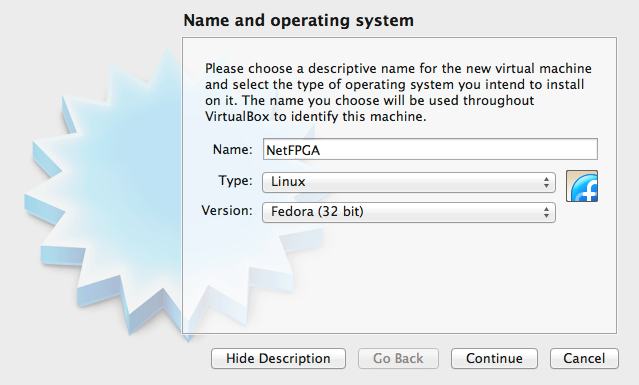
\includegraphics[scale=0.5]{figures/vm/vm1}
% \caption{Nome tipo e versão do sistema a ser instalado}
% \label{fig:vm.sys}
% \end{figure}

Instale o VirtualBox em seu sistema, execute-o e abra o tutorial
para criação de uma nova máquina virtual utilizando o menu
\emph{Machine $\rightarrow$ New}.  Escolha um nome para sua máquina
virtual (por exemplo, ``NetFPGA''), configure o tipo de máquina
virtual para ``Linux'' e a versão para ``Fedora (32 bit).''  No
passo seguinte, selecione a quantidade de memória desejada para a
máquina virtual.  Sugerimos pelo menos 3\,GiB para executar o Xilinx
ISE, mas você pode aumentar este valor se tiver memória disponível
no sistema hospedeiro.  Na próxima etapa, selecione a segunda opção
para criar um novo disco virtual (\emph{Create a virtual hard drive
now}).  Sugerimos o formato padrão para o disco virtual (VDI).
Sugerimos também utilização de alocação dinâmica de espaço para que
o disco virtual ocupe apenas o espaço necessário (\emph{Dynamically
allocated}).  Para finalizar esta etapa, indique o mesmo nome da
máquina virtual para facilitar a identificação do disco (por
exemplo, ``NetFPGA'') e selecione seu tamanho máximo.  É recomendado
selecionar um espaço razoável para o disco (pelo menos 20\,GB).
Como só será alocado o espaço necessário, aumentar o tamanho máximo
não implica custo.

% \begin{figure}[H]
% \centering
% 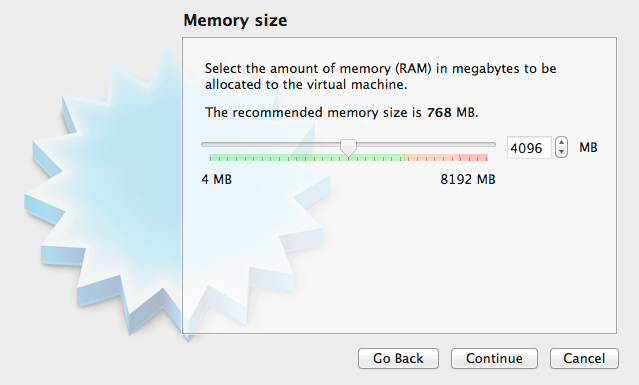
\includegraphics[scale=0.5]{figures/vm/vm2}
% \caption{Memória da máquina virtual}
% \label{fig:vm.mem}
% \end{figure}

% \begin{figure}[H]
% \centering
% 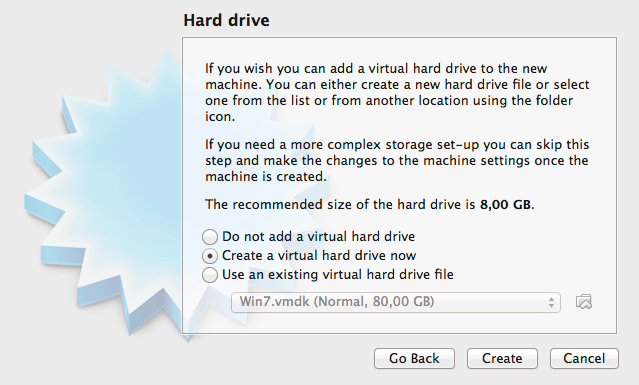
\includegraphics[scale=0.5]{figures/vm/vm3}
% \caption{Criar um novo disco virtual}
% \label{fig:vm.disk}
% \end{figure}

% \begin{figure}[H]
% \centering
% 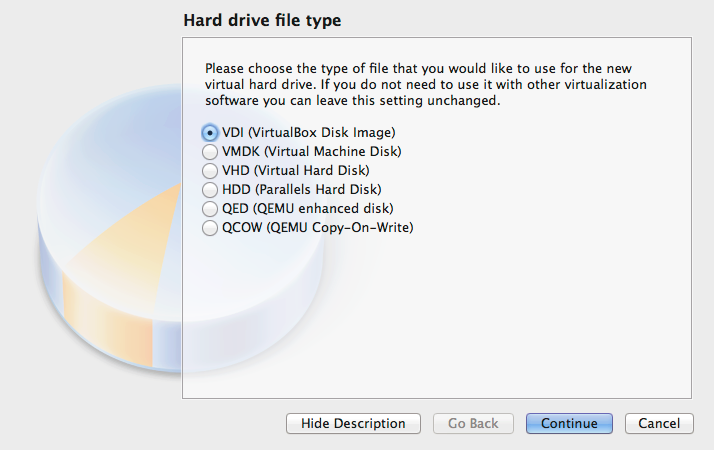
\includegraphics[scale=0.5]{figures/vm/vm4}
% \caption{Formato do disco virtual}
% \label{fig:vm.vdi}
% \end{figure}

% \begin{figure}[H]
% \centering
% 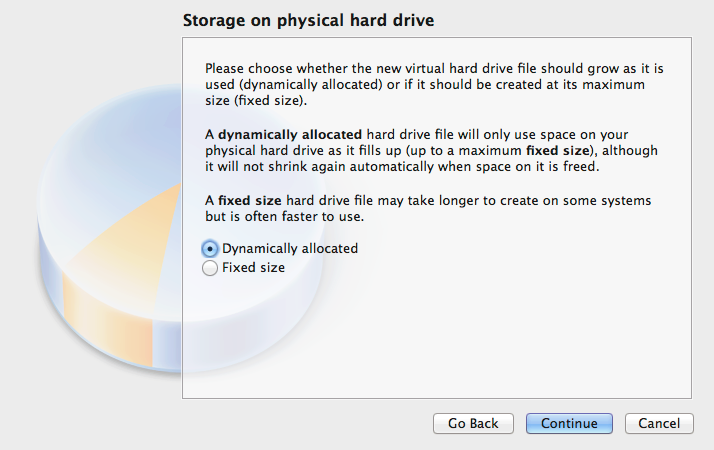
\includegraphics[scale=0.5]{figures/vm/vm5}
% \caption{Disco dinamicamente alocado}
% \label{fig:vm.dyn}
% \end{figure}

% \begin{figure}[H]
% \centering
% 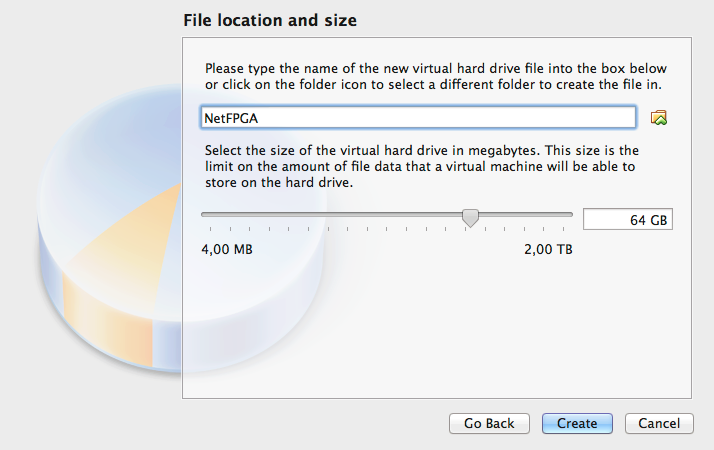
\includegraphics[scale=0.5]{figures/vm/vm6}
% \caption{Tamanho do disco virtual}
% \label{fig:vm.size}
% \end{figure}

% \begin{figure}[H]
% \centering
% 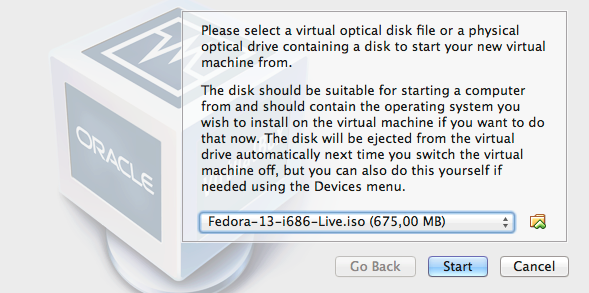
\includegraphics[scale=0.5]{figures/vm/vm7}
% \caption{Imagem para instalação do sistema}
% \label{fig:vm.cd}
% \end{figure}

Voltando à tela principal do VirtualBox, clique no botão
\emph{Start} para iniciar a máquina criada. Na primeira
inicialização o VirtualBox irá solicitar uma imagem de CD ou DVD de
instalação, indique o arquivo da imagem do Fedora 13. Os passos
seguintes são os mesmos, tanto para um sistema real quanto para a
máquina virtual.

\subsubsection{Instalação e configuração do sistema}
\label{ssec:linux}

% \begin{figure}[H]
% \centering
% 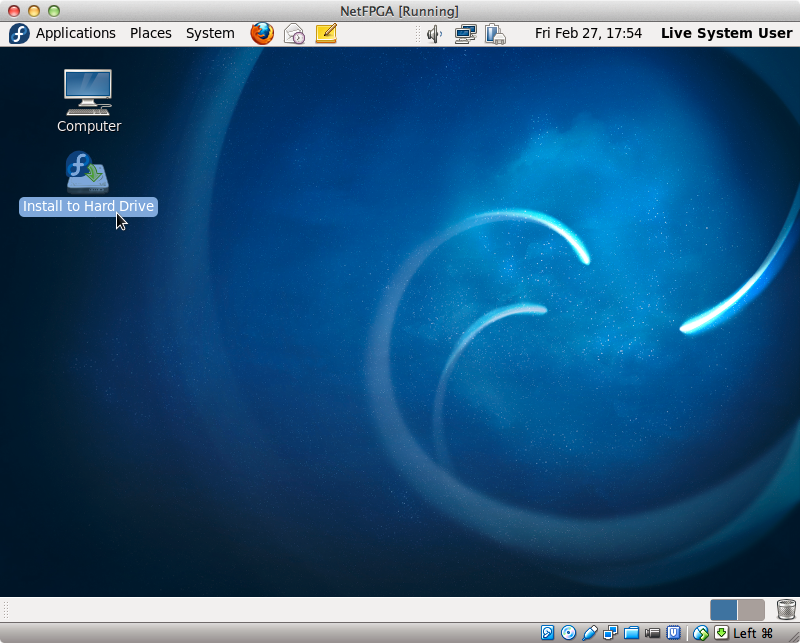
\includegraphics[scale=0.5]{figures/vm/vm8}
% \caption{Sistema inicializado a partir do CD/DVD Live}
% \label{fig:vm.live}
% \end{figure}

% \begin{figure}[!h]
% \centering
% 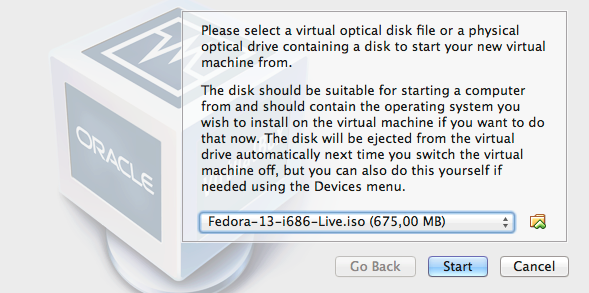
\includegraphics[scale=0.5]{figures/vm/vm7}
% \end{figure}

A inicialização a partir do CD ou DVD Live carrega o sistema para a
memória RAM, sem fazer qualquer alteração no disco. Após a
inicialização do sistema, selecione \emph{Install to hard drive}
para instalar o sistema no disco.  Siga os passos necessários para
selecionar o disco, determinar sua região e definir uma senha para o
superusuário (\emph{root}). Após finalizar a instalação, selecione o
comando de menu \emph{System $\rightarrow$ Shut Down} e reinicie o
computador (\emph{Restart}). Se estiver em uma máquina real, remova
o CD ou DVD da unidade. Se estiver em uma máquina virtual, desligue
o computador em vez de reiniciá-lo (\emph{Shut Down}), vá no
gerenciador de armazenamento (menu \emph{Settings $\rightarrow$
Storage}) e remova a imagem de CD ou DVD para iniciar a máquina
virtual a partir do disco virtual.

Após reiniciar o sistema é necessário informar mais algumas
configurações e criar uma conta de usuário. Para executar alguns dos
comandos usados neste minicurso é preciso ter acesso de superusuário
(\emph{root}), especialmente aqueles que fazem modificações no
sistema.  Por padrão, o Fedora não permite o \emph{login} como
\emph{root} no modo gráfico. Para contornar esta restrição é
possível usar o comando \ssf{su} que permite a um usuário comum
executar um \emph{shell} como \emph{root}. Se preferir modificar o
sistema para permitir o \emph{login} como \emph{root}, faça
\emph{login} na conta de usuário, acesse o diretório
\ssf{/etc/pam.d/} e edite os arquivos \ssf{gdm} e
\ssf{gdm-password}, comentando a seguinte linha em ambos:

\begin{verbnobox}[\small]
auth   required    pam_succeed_if.so user != root quiet
\end{verbnobox}

Os passos seguintes devem ser executados como \emph{root}, portanto
faça \emph{login} como \emph{root} ou use o comando \ssf{su} para
executar um \emph{shell} como \emph{root}.  A primeira modificação
necessária em nosso sistema é desabilitar o Security-Enhanced Linux
(SELinux). Para tal, edite o arquivo \ssf{/etc/selinux/config} e
mude a variável \ssf{SELINUX} para \ssf{disabled}.

A seguir, faremos a instalação de alguns pacotes necessários. Acesse
o diretório \ssf{/etc/yum.repos.d/} edite cada um dos arquivos com
extensão \ssf{.repo} trocando \ssf{https} das URLs por \ssf{http}.
Em seguida digite os seguintes comandos:

\begin{minted}{bash}
yum update
yum install gcc kernel-devel libnet-devel java-1.6.0-openjdk-devel
            python-argparse scapy wget iverilog gtkwave hping3 iperf
\end{minted}

Recomendamos também a instalação dos \emph{drivers} para o
VirtualBox através do menu \emph{Devices $\rightarrow$ Insert Guest
Additions CD Image}.

\subsubsection{Instalação das ferramentas}
\label{ssec:tools}

A seguir vamos configurar as ferramentas da Xilinx necessárias para
utilização com a NetFPGA.  Você precisará se registrar e obter
algumas licenças.  Faça o download do ISE Foundation 10.1 e depois
das atualizações para o Service Pack 3 do ISE Foundations e ISE IP
Update, todos para Linux 32-bit.  Após descompactar o pacote com o
ISE, a instalação pode ser feita executando o comando
\ssf{setup}.\footnote{A licença para esta ferramenta deve ser obtida
em \sssf{https://secure.xilinx.com/webreg/register.do?}
\sssf{group=9\_sw\_regid\_request}.  Selecione apenas ISE
Foundation.  Você receberá dois códigos, certifique-se de usar o
correto, pois a ferramenta alterna automaticamente para a versão
grátis se você usar o código errado (WebPACK).}

\begin{minted}{bash}
tar xvf ise_SFD.tar
ise/setup
\end{minted}

Escolha o caminho \ssf{/opt/Xilinx/10.1} para a instalação, mantenha
todas as opções selecionadas e aceite as licenças do
\emph{software}.  Depois da instalação, é preciso fazer a
atualização da ferramenta a partir dos arquivos baixados
anteriormente. Isso pode ser feito com os comandos abaixo.  Nos
instaladores é preciso apontar o caminho onde o ISE Foundation foi
instalado, \ssf{/opt/Xilinx/10.1/ISE}.

\begin{minted}{bash}
unzip 10_1_03_lin.zip
10_1_03_lin/setup
unzip ise_101_ip_update3_install.zip
ise_101_ip_update3_install/setup
\end{minted}

A plataforma NetFPGA 1G utiliza \emph{IP cores} da Xilinx que são
pagos, mas é possível obter uma licença de avaliação por 120 dias.
Ela permite simular os exemplos, sintetizar o \emph{hardware} e
testá-lo. Acesse \ssf{http://www.xilinx.com/getlicense/}, procure
por \emph{Evaluation and No Charge Cores} e clique em \emph{Search
Now}. A documentação da NetFPGA menciona os \emph{cores}
\ssf{DO-DI-PCI32-SP} e \ssf{DO-DI-TEMAC}, mas estes foram
descontinuados e substituídos pelos \emph{cores}
\ssf{EF-DI-PCI32-SP-PROJ} e \ssf{EF-DI-TEMAC-SITE},
respectivamente.\footnote{Acesse
\sssf{http://www.xilinx.com/support/documentation/customer\_notices/xcn09015.pdf}
para detalhes.} É preciso fazer a busca por estes códigos,
adicioná-los à licença desejada e gerar um único arquivo com os dois
itens. Durante o processo será solicitado um \emph{Host ID} que é a
identificação única do seu computador, neste caso a partir do
endereço físico da sua placa de rede principal. Num terminal do
Fedora 13 é possível obter este valor executando o programa
\ssf{ifconfig}.\footnote{Se sua placa de rede for identificada por
\sssf{eth1} ou \sssf{eth2} em vez de \sssf{eth0} será necessário
editar o arquivo \sssf{/etc/udev/rules.d/70-persistent-net.rules}
para fazer a correção.} Já na primeira linha o valor desejado
aparece depois de \ssf{HWaddr}.

\begin{verbnobox}[\small]
eth0      Link encap:Ethernet  HWaddr XX:XX:XX:XX:XX:XX
\end{verbnobox}

O arquivo obtido deve ser salvo em \ssf{/opt/Xilinx/Xilinx.lic}.
Adicione as seguintes linhas no arquivo \ssf{/root/.bashrc} para que
as ferramentas fiquem disponíveis no caminho do sistema e para que
encontrem o arquivo de licenças:

\begin{minted}{bash}
export LM_LICENSE_FILE=/opt/Xilinx/Xilinx.lic
source /opt/Xilinx/10.1/ISE/settings32.sh
\end{minted}

Finalmente, para instalar o software da NetFPGA e reiniciar o
sistema usamos a seguinte sequência de comandos.  Estes comandos
irão configurar um novo repositório no Fedora.  A instalação do
pacote \ssf{netfpga-base} irá instalar várias outras dependências
necessárias para utilização do \emph{software} da NetFPGA.

\begin{verbnobox}[\small]
rpm -Uhv http://netfpga.org/yum/el5/RPMS/noarch/netfpga-repo-1-1_CentOS5.noarch.rpm
yum install netfpga-base
/usr/local/netfpga/lib/scripts/user_account_setup/user_account_setup.pl
reboot
\end{verbnobox}

Após a reinicialização digite a seguinte sequência no terminal para
concluir a instalação.  Esta sequência irá preparar arquivos
necessários para funcionamento do pacote de \emph{software} da
NetFPGA.

\begin{verbnobox}[\small]
cd /root/netfpga
make
make install
\end{verbnobox}

Para fazer simulações de alguns exemplos é necessário baixar modelos
de simulação das memórias presentes na placa. Para tal, edite e
execute o seguinte programa, substituindo antes a URL na linha 20
por
{\small\url{http://www.dcc.ufmg.br/~cunha/netfpga/256Mb_ddr2.zip}}.

\begin{minted}{bash}
/root/netfpga/lib/scripts/fetch_mem_models/fetch_mem_models.pl
\end{minted}

\newpage

Se tudo estiver configurado adequadamente o comando a seguir deve
executar a simulação de um dos exemplos disponíveis:

\begin{minted}{bash}
nf_test.py --isim --major loopback --minor crc sim
\end{minted}

Este comando simulará o projeto apontado pela variável
\ssf{NF\_DESIGN\_DIR} enviando pacotes de tamanhos variáveis para as
quatro interfaces da NetFPGA, ligadas em \ssf{loopback}. A primeira
execução pode levar um longo tempo se os módulos precisarem ser
sintetizados.  Detalharemos o sistema de destes da plataforma NetFPGA na
\secstr~\ref{sec:impl.test}.

\subsection{Utilização do \emph{firewall} exemplo: passo-a-passo}


Descompacte o pacote de \emph{software} disponibilizado neste
projeto.\footnotemark{} O pacote já contém a imagem que deve ser
gravada na NetFPGA para configurá-la como uma placa de rede com um
\emph{firewall} integrado capaz de filtrar pacotes destinados a
portas TCP específicas.  Entre no diretório que contém as imagens de
projetos que podem ser gravadas na NetFPGA e utilize o programa
\ssf{nf\_download} para realizar a gravação.

\footnotetext{Você pode obter o pacote no site do tutorial:
\sssf{http://www.dcc.ufmg.br/~cunha/netfpga/}.}

\begin{minted}{bash}
cd /root/netfpga/bitfiles
nf_download firewall.bit
\end{minted}

Se quiser sintetizar novamente a imagem do \emph{firewall} que é
gravada na NetFPGA, basta executar os seguintes comandos.  Este
processo é demorado e não é necessário.

\begin{minted}{bash}
cd /root/netfpga/projects/firewall/synth
make
\end{minted}

Após execução do programa \ssf{nf\_download} a NetFPGA está
programada como quatro interfaces de rede capazes de descartar
pacotes TCP dependendo das portas de destino.  Pode-se configurar a
interface de rede para funcionar normalmente no Linux usando
comandos como \ssf{ifconfig}.

\begin{verbnobox}[\small]
ifconfig nf2c0 10.0.0.1 netmask 255.0.0.0
\end{verbnobox}

Para testar a placa, iremos utilizar o programa \ssf{hping3}.  O
programa \ssf{hping3} permite gerar pacotes TCP para uma porta de
destino passada como parâmetro.

\begin{verbnobox}[\small]
hping3 -p 5151 10.0.0.2
\end{verbnobox}

O parâmetro 10.0.0.2 é o endereço IP de destino de outro computador
alcançável por uma das interfaces da NetFPGA.  O destino
provavelmente responderá os pacotes enviados pelo \ssf{hping3} com
pacotes ICMP \emph{port unreachable} (porta não alcançável) ou com
pacotes com o \emph{flag} de \emph{reset} ligado.\footnotemark{}

\footnotetext{O computador com IP 10.0.0.2 pode não responder com um
pacote ICMP \emph{port unreachable} ou TCP \emph{reset} caso esteja
com a porta 5151 aberta.  Neste caso basta utilizar outro número de
porta.  O computador também pode não enviar respostas ICMP
\emph{port unreachable} se estiver configurado para não enviar
pacotes ICMP para esse tipo de erro.}

É possível monitorar o fluxo de pacotes na interface de rede
utilizando programas como \ssf{wireshark} ou \ssf{tcpdump}.  Estes
programas capturam e mostram o conteúdo de todos os pacotes numa
interface de rede.  Pode-se executar o \ssf{tcpdump} na interface
\ssf{nf2c0} para verificar que os pacotes TCP enviados pelo
\ssf{hping3} e as respostas de TCP \emph{reset} estão passando pela
interface.

\begin{verbnobox}[\small]
tcpdump -i eth0 -n host 10.0.0.1 and port 5151 -vv
...
12:24:21.326608 IP (ttl 63, id 20588, flags [none], proto TCP (6), length 40)
    10.0.0.1.50082 > 10.0.0.2.5151: Flags [none], cksum 0x6245 (correct),
                seq 519591940, win 512, length 0
12:24:21.326635 IP (ttl 64, id 0, flags [DF], proto TCP (6), length 40)
    10.0.0.2.5151 > 10.0.0.1.50084: Flags [R.], cksum 0xb6d7 (correct),
                seq 0, ack 1680124174, win 0, length 0
...
\end{verbnobox}

O \ssf{tcpdump} permite a visualização do conteúdo dos pacotes
transmitidos pelo \ssf{hping3} e as respostas do outro computador.
Observamos, por exemplo, que o tempo de vida (TTL, \emph{time to
live}) das sondas (primeiro pacote) têm TTL 63.  Isto acontece por
que nosso \emph{firewall} decrementa o TTL de pacotes TCP que passam
pelas interfaces. Isso ilustra a possibilidade de modificar pacotes
em tempo de processamento sem sacrificar banda de rede, como será
detalhado na \secstr~\ref{sec:impl.mod}.

Para verificar o correto funcionamento do \emph{firewall}, pode-se
configurar a NetFPGA para filtrar todos os pacotes TCP com porta
5151.  Para isso, disponibilizamos o programa de usuário chamado
\ssf{nffw} que configura quais portas devem ser filtradas. O
\emph{firewall} de exemplo suporta filtrar até quatros portas
distintas.

\begin{minted}{text}
nffw 5151 22 25 80
\end{minted}

Depois da execução do \ssf{nffw}, a NetFPGA filtrará todos os
pacotes TCP com porta de destino 5151, 22, 25 e 80.  A NetFPGA não
transmitirá os pacotes TCP gerados pelo \ssf{hping3} ao destino, o
que pode ser verificado executando o \ssf{tcpdump} no destino.  Como
o destino não recebe as sondas geradas pelo \ssf{hping3}, ele não
responderá com pacotes TCP \emph{reset}, o que é visível nas saídas
do \ssf{tcpdump} e \ssf{hping3} executando no computador com a
NetFPGA.  Note que o \ssf{tcpdump} na interface \ssf{nf2c0} continua
mostrando os pacotes enviados pelo \ssf{hping3}.  Isto acontece
porque o \ssf{tcpdump} funciona em cooperação com o Linux.  A
filtragem e descarte do pacote só acontece depois do Linux passar o
pacote para processamento no \emph{hardware} da NetFPGA, onde o
Linux não tem mais visibilidade nem controle sobre o processamento
do pacote.

Pode-se reconfigurar o \emph{firewall} na NetFPGA dinamicamente
reexecutando o comando \ssf{nffw}.  Como exemplificado acima, as
configurações podem ser testadas utilizando programas como
\ssf{hping3} e \ssf{tcpdump}.

Também realizamos testes com o \ssf{iperf}, que faz troca
bidirecional de pacotes. Configuramos a máquina com a NetFPGA com o
\emph{firewall} e o outro computador com um adaptador comum. Usamos
o computador com a NetFPGA como cliente e o outro computador como
servidor. Os pacotes serão enviados através da porta 5001 padrão do
\ssf{iperf}.  No servidor executamos \ssf{iperf -s}; no cliente
observamos:

\begin{verbnobox}[\small]
iperf -c 10.0.0.2 -i 1
------------------------------------------------------------
Client connecting to 10.0.0.2, TCP port 5001
TCP window size: 16.0 KByte (default)
------------------------------------------------------------
[  3] local 10.0.0.1 port 43905 connected with 10.0.0.2 port 5001
[ ID] Interval       Transfer     Bandwidth
[  3]  0.0- 1.0 sec  49.4 MBytes   414 Mbits/sec
[  3]  1.0- 2.0 sec  49.0 MBytes   411 Mbits/sec
[  3]  2.0- 3.0 sec  49.4 MBytes   414 Mbits/sec
[  3]  3.0- 4.0 sec  12.1 MBytes   102 Mbits/sec
[  3]  4.0- 5.0 sec  0.00 Bytes  0.00 bits/sec
[  3]  5.0- 6.0 sec  0.00 Bytes  0.00 bits/sec
[  3]  6.0- 7.0 sec  0.00 Bytes  0.00 bits/sec
[  3]  7.0- 8.0 sec  0.00 Bytes  0.00 bits/sec
[  3]  8.0- 9.0 sec  0.00 Bytes  0.00 bits/sec
[  3]  9.0-10.0 sec  0.00 Bytes  0.00 bits/sec
\end{verbnobox}

Após três segundos executamos o \ssf{nffw} para bloquear todo o
tráfego com porta TCP de destino 5001.  Vemos que o tráfego é
bloqueado instantaneamente. Na próxima seção iremos descrever a
arquitetura da NetFPGA, conceitos que servirão de base para a
implementação passo-a-passo do \emph{firewall} na
\secstr~\ref{sec:impl}.
